\documentclass{article}
\usepackage{amsmath}
\usepackage{amssymb}
\usepackage[dvipsnames]{xcolor}
\usepackage{graphicx}
\usepackage{tikz}
\usepackage{pgfplots}
\usetikzlibrary{arrows}
\usetikzlibrary{datavisualization.formats.functions}
\usepgfplotslibrary{fillbetween}
\usetikzlibrary{patterns}
\usepackage[margin=1.2in]{geometry}


\begin{document}

\title{Theory of Probability HW \#0}
\author{Ozaner Hansha}
\date{September 9, 2019}
\maketitle

\newcommand*\Eval[3]{\left[#1\right]_{#2}^{#3}}

\section*{Problem 1}
\noindent\textbf{Problem:} Compute the following infinite sum:

$$\sum_{i=0}^\infty\left(\frac{2}{3}\right)^{2i+4}=\left(\frac{2}{3}\right)^4+\left(\frac{2}{3}\right)^6+\left(\frac{2}{3}\right)^8+\cdots$$

\noindent\textbf{Solution:} After splitting up the general term of the series into two factors, it becomes clear that it is a geometric series with $\left(\frac{2}{3}\right)^4$ as the principal term, and $\left(\frac{2}{3}\right)^2$ as the common ratio. As such, the series is given by the following formula:

$$\sum_{i=0}^\infty\left(\frac{2}{3}\right)^{2i+4}=\sum_{i=0}^\infty\left(\frac{2}{3}\right)^4\left(\frac{2}{3}\right)^{2i}=\frac{\left(\frac{2}{3}\right)^4}{1-\left(\frac{2}{3}\right)^2}=\frac{16}{45}$$

\section*{Problem 2}
\noindent\textbf{Problem a:} Evaluate the following indefinite integral:

$$\int x^2e^{\frac{2x}{5}}\, dx$$

\noindent\textbf{Solution:} We can solve this by using integration of parts twice over. Where integration by parts is given by the following identity:

$$\int u\,dv=uv-\int v\,du$$

We begin by letting $u=x^2$ and $v=e^{\frac{2x}{5}}$. Differentiating, we arrive at the following:

\begin{gather*}
    \frac{du}{dx}=2x\rightarrow du=2x\,dx\\
    \frac{dv}{dx}=\frac{2}{5}e^{\frac{2x}{5}}\rightarrow dv=\frac{2}{5}e^{\frac{2x}{5}}\,dx
\end{gather*}

Plugging this into the identity we have:
\begin{align*}
    \int \frac{2}{5}x^2e^{\frac{2x}{5}}\,dx&=x^2e^{\frac{2x}{5}}-\int 2xe^{\frac{2x}{5}}\,dx\\
    \frac{2}{5}\int x^2e^{\frac{2x}{5}}\,dx&=x^2e^{\frac{2x}{5}}-2\int xe^{\frac{2x}{5}}\,dx\\
    \implies\underbrace{\int x^2e^{\frac{2x}{5}}\,dx}_{\text{Original Integral}}&=\frac{5}{2}(x^2e^{\frac{2x}{5}}-2\int xe^{\frac{2x}{5}}\,dx)\\
    &=\frac{5}{2}x^2e^{\frac{2x}{5}}-5\underbrace{\int xe^{\frac{2x}{5}}\,dx}_{\text{New Integral}}
\end{align*}

As we can see we are very close to solving the original integral, we just need to use integration by parts one more time to solve the new integral bracketed above. And so we'll do just that, let $u=x$ and once again $v=e^{\frac{2x}{5}}$. Differentiating, we get:

\begin{gather*}
    \frac{du}{dx}=1\rightarrow du=\,dx\\
    \frac{dv}{dx}=\frac{2}{5}e^{\frac{2x}{5}}\rightarrow dv=\frac{2}{5}e^{\frac{2x}{5}}\,dx
\end{gather*}

Plugging this into the identity we get:

\begin{align*}
    \int \frac{2}{5}xe^{\frac{2x}{5}}\,dx&=xe^{\frac{2x}{5}}-\int e^{\frac{2x}{5}}\,dx\\
    \frac{2}{5}\int xe^{\frac{2x}{5}}\,dx&=xe^{\frac{2x}{5}}-\int e^{\frac{2x}{5}}\,dx\\
    \underbrace{\int xe^{\frac{2x}{5}}\,dx}_{\text{New Integral}}&=\frac{5}{2}(xe^{\frac{2x}{5}}-\int e^{\frac{2x}{5}}\,dx)\\
    &=\frac{5}{2}(xe^{\frac{2x}{5}}-\frac{5}{2}e^{\frac{2x}{5}}+C_1)\\
    &=\frac{5}{2}xe^{\frac{2x}{5}}-\left(\frac{5}{2}\right)^2e^{\frac{2x}{5}}+C_2
\end{align*}

Now plugging the new integral into our equation for our original integral we finally have:

\begin{align*}
    \int x^2e^{\frac{2x}{5}}\,dx&=\frac{5}{2}x^2e^{\frac{2x}{5}}-5\left(\frac{5}{2}xe^{\frac{2x}{5}}-\left(\frac{5}{2}\right)^2e^{\frac{2x}{5}}+C_2\right)\\
    &=\frac{5}{2}x^2e^{\frac{2x}{5}}-\frac{25}{2}xe^{\frac{2x}{5}}+\frac{125}{4}e^{\frac{2x}{5}}+C_3\\
    &=\frac{5}{4}e^{\frac{2x}{5}}\left(2x^2-10x+25\right)+C_3
\end{align*}

Where $C_3\in\mathbb R$. With this we are done.
\\\\

\noindent\textbf{Problem b:} Evaluate the following integral:
$$\int_{-\infty}^\infty xe^{\frac{-x^2}{2}}\, dx$$

\noindent\textbf{Solution:} First we need to evaluate the indefinite form of the above integral. We do this via\\ $u$-substitution with:
\begin{gather*}
    u=\frac{-x^2}{2}\\
    \frac{du}{dx}=-x\rightarrow dx=-\frac{du}{x}
\end{gather*}

Plugging these into the indefinite integral we find:

\begin{align*}
    \int xe^{\frac{-x^2}{2}}\, dx &= \int \frac{-xe^u\, du}{x}\\
    &= -\int e^u\, du\\
    &=-e^u+C=-e^{\frac{-x^2}{2}}+C
\end{align*}

We can now evaluate the definite integral via the following chain of equalities:

\begin{align*}
    \int_{-\infty}^\infty xe^{\frac{-x^2}{2}}\, dx&=\int_{-\infty}^0 xe^{\frac{-x^2}{2}}\, dx+\int_0^\infty xe^{\frac{-x^2}{2}}\, dx\\
    &=\lim_{t\to-\infty}\int_t^0 xe^{\frac{-x^2}{2}}\, dx+\lim_{t\to\infty}\int_0^t xe^{\frac{-x^2}{2}}\, dx\\
    &=\lim_{t\to-\infty}\Eval{-e^{\frac{-x^2}{2}}}{t}{0}+\lim_{t\to\infty}\Eval{-e^{\frac{-x^2}{2}}}{0}{t}\\
    &=\lim_{t\to-\infty}\left(-1+e^{\frac{-t^2}{2}}\right)+\lim_{t\to\infty}\left(-e^{\frac{-t^2}{2}}+1\right)\\
    &=-1+1=0
\end{align*}
\indent And we are done.

\section*{Problem 3}
\noindent\textbf{Problem:} Evaluate the following integral:

$$\int\int_D x+y\,dxdy$$

Where $D$ is the set of all points such that $3x+y\le 3$, $x+y\ge 1$ and $x\ge y$.
\\

\noindent\textbf{Solution:} First off, solving for $y$ in these inequalities will help both in graphing them, as well as calculating the bounds for our integral:
\begin{align*}
    3x+y\le 3\rightarrow y&\le 3-3x\\
    x+y\ge 1\rightarrow y&\ge 1-x\\
    x\ge y\rightarrow y&\le x
\end{align*}

Using these, we can shade the area of the plane that satisfies all 3 conditions:

\begin{center}
    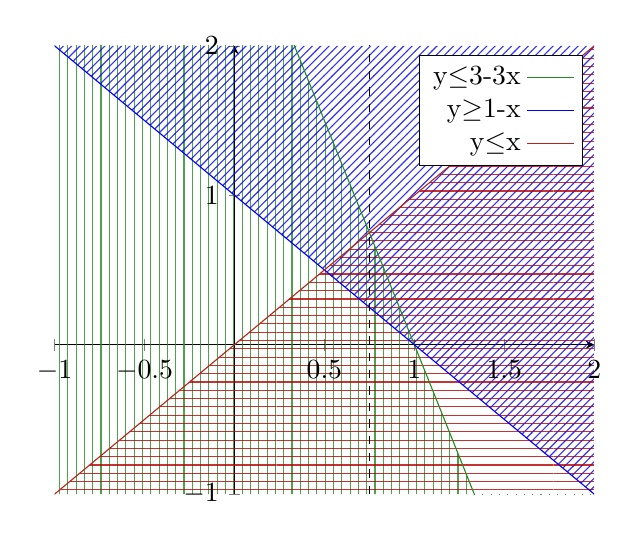
\begin{tikzpicture}
    \begin{axis}[
        xmin=-1,xmax=2,
        ymin=-1,ymax=2,
        axis lines=center,
        legend style={legend cell align=right,legend plot pos=right}]
    
    \plot[name path=C, thick,samples=100,domain=-1:2,
        forget plot,draw=none] {3-3*x};
    \plot[name path=D,thick,samples=100,domain=-1:2,
        forget plot,draw=none] {-1};
    \addplot[fill=ForestGreen,
        opacity=.8,
        forget plot,
        pattern=vertical lines,
        pattern color=ForestGreen]
        fill between [of=D and C, soft clip={domain=-1:2}];
    
    \plot[name path=A, thick,samples=100,domain=-1:2,
        forget plot,draw=none] {1-x};
    \plot[name path=B,thick,samples=100,domain=-1:2,
        forget plot,draw=none] {2};
    \addplot[fill=blue,
        opacity=.8,
        forget plot,
        pattern=north east lines,
        pattern color=blue]
        fill between [of=A and B, soft clip={domain=-1:2}];
    
    \plot[name path=C, thick,samples=100,domain=-1:2,
        forget plot,draw=none] {x};
    \plot[name path=D,thick,samples=100,domain=-1:2,
        forget plot,draw=none] {-1};
    \addplot[fill=BrickRed,
        opacity=.8,
        forget plot,
        pattern=horizontal lines,
        pattern color=BrickRed]
        fill between [of=D and C, soft clip={domain=-1:2}];    
    \addplot[color=ForestGreen,domain=-4:4,samples=100] {3-3*x};
    \addlegendentry{y$\le$3-3x}
    \addplot[color=blue,domain=-4:4,samples=100] {1-x};
    \addlegendentry{y$\ge$1-x}
    \addplot[color=BrickRed,domain=-4:4,samples=100] {x};
    \addlegendentry{y$\le$x}
    \end{axis}
    \draw [dashed] (4,0) -- (4,5.7);
    \end{tikzpicture}
\end{center}

Integrating with respect to $y$ first, we can see there are two distinct triangle to integrate, each separated by the dashed black line. For the triangle on the left, the bounds of integration for $y$ start from the blue line ($y=1-x$) to the red line ($y=x$). For the triangle on the right, the bounds again start from the blue line but end at the green line ($y=3-3x$) making our integral thus far:

$$\int^?_?\int^{x}_{1-x}x+y\,dydx+\int^?_?\int^{3-3x}_{1-x}x+y\,dydx$$

For the left triangle the bounds of integration over $x$ begin where the red and blue lines intersect, and end where the red and green lines intersect. For the right triangle they begin where the left triangle ends and end where the blue and green lines intersect. These intersection points are given by:

\begin{align*}
    \textcolor{blue}{1-x}=\textcolor{BrickRed}{x}&\rightarrow x=\frac{1}{2}\\
    \textcolor{ForestGreen}{3-3x}=\textcolor{BrickRed}{x}&\rightarrow x=\frac{3}{4}\\
    \textcolor{blue}{1-x}=\textcolor{ForestGreen}{3-3x}&\rightarrow x=1
\end{align*}

And so our integral is given by the following:

$$\int^{\frac{3}{4}}_\frac{1}{2}\int^{x}_{1-x}x+y\,dydx+\int^{1}_{\frac{3}{4}}\int^{3-3x}_{1-x}x+y\,dydx$$
\pagebreak

All that's left is to evaluate it. We'll start with the left triangle:

\begin{align*}
    \int^\frac{3}{4}_\frac{1}{2}\int^{x}_{1-x}x+y\,dydx&=\int^\frac{3}{4}_\frac{1}{2}\Eval{\frac{y^2}{2}+xy}{1-x}{x}\,dx\\
    &=\int^\frac{3}{4}_\frac{1}{2}\frac{x^2}{2}+x^2-\left(\frac{(1-x)^2}{2}+x(1-x)\right)\,dx\\
    &=\int^\frac{3}{4}_\frac{1}{2}\frac{3x^2}{2}-\frac{1}{2}+x-\frac{x^2}{2}-x+x^2\,dx\\
    &=\int^\frac{3}{4}_\frac{1}{2}2x^2-\frac{1}{2}\,dx\\
    &=\Eval{\frac{2x^3}{3}-\frac{x}{2}}{\frac{1}{2}}{\frac{3}{4}}\\
    &=\left(\frac{9}{32}-\frac{3}{8}\right)-\left(\frac{1}{12}-\frac{1}{4}\right)=\frac{7}{96}
\end{align*}

And for the right triangle we have:

\begin{align*}
    \int^{1}_{\frac{3}{4}}\int^{3-3x}_{1-x}x+y\,dydx&=\int^1_\frac{3}{4}\Eval{\frac{y^2}{2}+xy}{1-x}{3-3x}\,dx\\
    &=\int^\frac{3}{4}_\frac{1}{2}3x(1-x)-x(1-x)+\left(\frac{(3-3x)^2}{2}-\left(\frac{1-x}{2}\right)^2\right)\,dx\\
    &=\int^1_\frac{3}{4}2x-2x^2+(4-8x+4x^2)\,dx\\
    &=\int^1_\frac{3}{4}2x^2-6x+4\,dx\\
    &=\Eval{\frac{2x^3}{3}-3x^2+4x}{\frac{3}{4}}{1}\\
    &=\left(\frac{2}{3}-3+4\right)-\left(\frac{3}{8}-\frac{27}{16}+3\right)=\frac{7}{96}
\end{align*}

Putting these together, our final answer is:

$$\frac{7}{96}+\frac{7}{96}=\frac{7}{48}$$

\section*{Problem 4}
\noindent\textbf{Problem:} Rewrite the following integral with the order of integration reversed:

$$\int_0^\infty\int_{2y}^\infty f(x,y)\,dxdy$$
\pagebreak

\noindent\textbf{Solution:} When we draw the area of integration in its current form we get the graph on the left:

% In the pic it should be y\in[0,x/2] for the second graph since the y is less than 0 for x<0

\begin{center}
    \scalebox{.95}{
        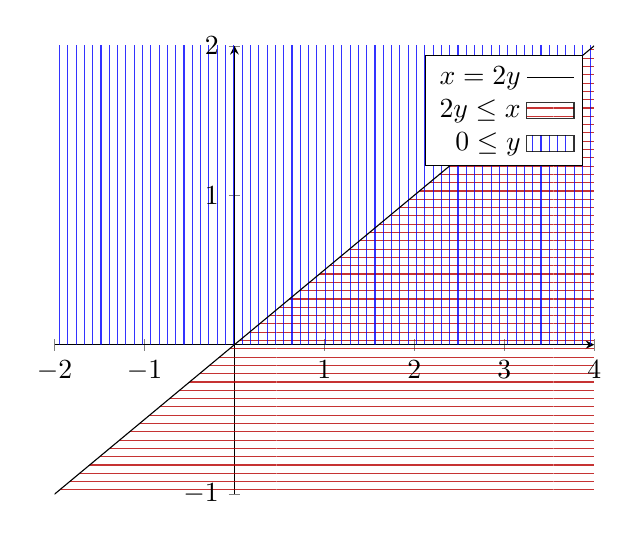
\begin{tikzpicture}
            \begin{axis}[
                xmin=-2,xmax=4,
                ymin=-1,ymax=2,
                axis lines=center,
                legend style={legend cell align=right,legend plot pos=right}]
            
            \addplot[color=black,domain=-4:4,samples=100] {x/2};
            \addlegendentry{$x=2y$}

            \plot[name path=C, thick,samples=100,domain=-2:4,
                forget plot,draw=none] {x/2};
            \plot[name path=D,thick,samples=100,domain=-2:4,
                forget plot,draw=none] {-1};
            \addplot[fill=BrickRed,
                opacity=.8,
                pattern=horizontal lines,
                pattern color=BrickRed]
                fill between [of=D and C, soft clip={domain=-2:4}];
            \addlegendentry{$2y\le x$}

            \plot[name path=A, thick,samples=100,domain=-2:4,
                forget plot,draw=none] {4};
            \plot[name path=B,thick,samples=100,domain=-2:4,
                forget plot,draw=none] {0};
            \addplot[fill=blue,
                opacity=.8,
                pattern=vertical lines,
                pattern color=blue]
                fill between [of=A and B, soft clip={domain=-2:4}];
            \addlegendentry{$0\le y$}

            \end{axis}
        \end{tikzpicture}

        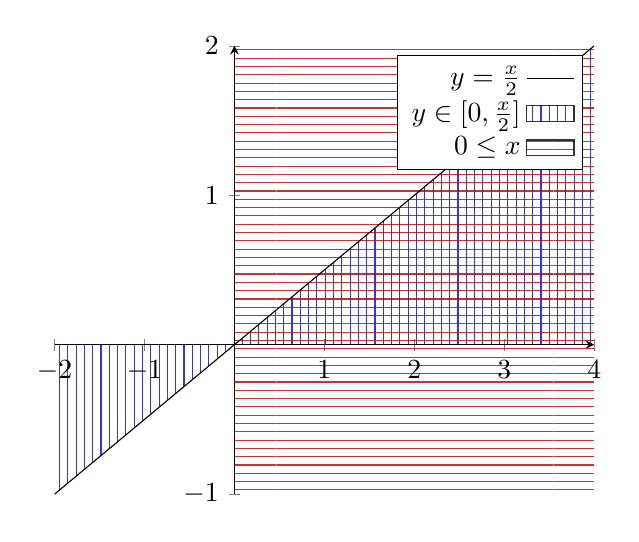
\begin{tikzpicture}
            \begin{axis}[
                xmin=-2,xmax=4,
                ymin=-1,ymax=2,
                axis lines=center,
                legend style={legend cell align=right,legend plot pos=right}]
            
            \addplot[color=black,domain=-4:4,samples=100] {x/2};
            \addlegendentry{$y=\frac{x}{2}$}
        
            \plot[name path=A, thick,samples=100,domain=-2:4,
                forget plot,draw=none] {x/2};
            \plot[name path=B,thick,samples=100,domain=-2:4,
                forget plot,draw=none] {0};
            \addplot[fill=blue,
                opacity=.8,
                pattern=vertical lines,
                pattern color=blue]
                fill between [of=A and B, soft clip={domain=-2:4}];
            % \addlegendentry{$0\le y\le\frac{x}{2}$}
            \addlegendentry{$y\in[0,\frac{x}{2}]$}
            
            \plot[name path=C, thick,samples=100,domain=-2:4,
                forget plot,draw=none] {2};
            \plot[name path=D,thick,samples=100,domain=-2:4,
                forget plot,draw=none] {-1};
            \addplot[fill=BrickRed,
                opacity=.8,
                pattern=horizontal lines,
                pattern color=BrickRed]
                fill between [of=C and D, soft clip={domain=0:4}];
            \addlegendentry{$0\le x$}
        
            \end{axis}
        \end{tikzpicture}
    }
\end{center}

As we can see, the bounds of the graphs above overlap in the same area. And so by inspection, we have that the two definite integrals below are equivalent:

$$\int_0^\infty\int_{2y}^\infty f(x,y)\,dxdy=\int_0^\infty\int_{0}^{\frac{x}{2}} f(x,y)\,dydx$$

\section*{Problem 5}
\noindent\textbf{Problem:} Compute $\frac{\partial f}{\partial y}$ for the following function $f$:

$$f(x,y)=\frac{e^{\frac{-x}{y}}e^{-y}}{y}$$

\noindent\textbf{Solution:} We can compute the desired partial derivative of $f$ by using the product and the chain rules:

\begin{align*}
    \frac{\partial}{\partial y}\left(\frac{e^{\frac{-x}{y}}e^{-y}}{y}\right)&=\frac{\partial}{\partial y}\left(\frac{1}{y}\cdot e^{\frac{-x}{y}-y}\right)\\
    &=\frac{1}{y}\cdot\frac{\partial}{\partial y}\left(e^{\frac{-x}{y}-y}\right)+e^{\frac{-x}{y}-y}\cdot\frac{\partial}{\partial y}\left(\frac{1}{y}\right)\\
    &=\frac{e^{\frac{-x}{y}-y}}{y}\frac{\partial}{\partial y}\left(\frac{-x}{y}-y\right)-\frac{e^{\frac{-x}{y}-y}}{y^2}\\
    &=\frac{-e^{\frac{-x}{y}-y}}{y}\left(\frac{x}{y^2}+1\right)-\frac{e^{\frac{-x}{y}-y}}{y^2}\\
    &=\frac{1}{ye^{\frac{x}{y}+y}}\left(\frac{x}{y^2}-\frac{1}{y}-1\right)
\end{align*}

And we are done.

\end{document}